% Options for packages loaded elsewhere
\PassOptionsToPackage{unicode}{hyperref}
\PassOptionsToPackage{hyphens}{url}
%
\documentclass[
]{article}
\usepackage{lmodern}
\usepackage{amssymb,amsmath}
\usepackage{ifxetex,ifluatex}
\ifnum 0\ifxetex 1\fi\ifluatex 1\fi=0 % if pdftex
  \usepackage[T1]{fontenc}
  \usepackage[utf8]{inputenc}
  \usepackage{textcomp} % provide euro and other symbols
\else % if luatex or xetex
  \usepackage{unicode-math}
  \defaultfontfeatures{Scale=MatchLowercase}
  \defaultfontfeatures[\rmfamily]{Ligatures=TeX,Scale=1}
\fi
% Use upquote if available, for straight quotes in verbatim environments
\IfFileExists{upquote.sty}{\usepackage{upquote}}{}
\IfFileExists{microtype.sty}{% use microtype if available
  \usepackage[]{microtype}
  \UseMicrotypeSet[protrusion]{basicmath} % disable protrusion for tt fonts
}{}
\makeatletter
\@ifundefined{KOMAClassName}{% if non-KOMA class
  \IfFileExists{parskip.sty}{%
    \usepackage{parskip}
  }{% else
    \setlength{\parindent}{0pt}
    \setlength{\parskip}{6pt plus 2pt minus 1pt}}
}{% if KOMA class
  \KOMAoptions{parskip=half}}
\makeatother
\usepackage{xcolor}
\IfFileExists{xurl.sty}{\usepackage{xurl}}{} % add URL line breaks if available
\IfFileExists{bookmark.sty}{\usepackage{bookmark}}{\usepackage{hyperref}}
\hypersetup{
  pdftitle={SFBay Rocky Shore Survey analyses},
  pdfauthor={Karina J. Nielsen},
  hidelinks,
  pdfcreator={LaTeX via pandoc}}
\urlstyle{same} % disable monospaced font for URLs
\usepackage[margin=1in]{geometry}
\usepackage{longtable,booktabs}
% Correct order of tables after \paragraph or \subparagraph
\usepackage{etoolbox}
\makeatletter
\patchcmd\longtable{\par}{\if@noskipsec\mbox{}\fi\par}{}{}
\makeatother
% Allow footnotes in longtable head/foot
\IfFileExists{footnotehyper.sty}{\usepackage{footnotehyper}}{\usepackage{footnote}}
\makesavenoteenv{longtable}
\usepackage{graphicx,grffile}
\makeatletter
\def\maxwidth{\ifdim\Gin@nat@width>\linewidth\linewidth\else\Gin@nat@width\fi}
\def\maxheight{\ifdim\Gin@nat@height>\textheight\textheight\else\Gin@nat@height\fi}
\makeatother
% Scale images if necessary, so that they will not overflow the page
% margins by default, and it is still possible to overwrite the defaults
% using explicit options in \includegraphics[width, height, ...]{}
\setkeys{Gin}{width=\maxwidth,height=\maxheight,keepaspectratio}
% Set default figure placement to htbp
\makeatletter
\def\fps@figure{htbp}
\makeatother
\setlength{\emergencystretch}{3em} % prevent overfull lines
\providecommand{\tightlist}{%
  \setlength{\itemsep}{0pt}\setlength{\parskip}{0pt}}
\setcounter{secnumdepth}{5}

\title{SFBay Rocky Shore Survey analyses}
\author{Karina J. Nielsen}
\date{Last compiled on 01 January 2021}

\begin{document}
\maketitle

{
\setcounter{tocdepth}{2}
\tableofcontents
}
\hypertarget{dataviz-of-sfbay-quadrat-surveys}{%
\section{Dataviz of sfbay quadrat surveys}\label{dataviz-of-sfbay-quadrat-surveys}}

\hypertarget{rockweed-fucus-distichus}{%
\subsection{\texorpdfstring{Rockweed, \emph{Fucus distichus}}{Rockweed, Fucus distichus}}\label{rockweed-fucus-distichus}}

\begin{figure}

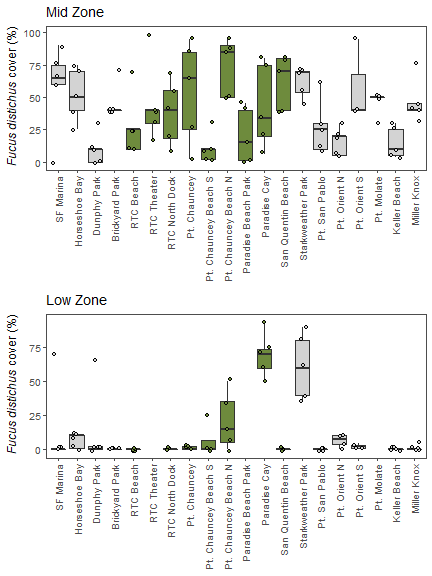
\includegraphics{sfb_quadrats_files/figure-latex/rockweed-by-zone-site-fig-1} \hfill{}

\caption{ Rockweed (Fucus distichus) cover in the mid and low intertidal at survey sites. Colored fill indicates reference sites for RTC restoration planning.}\label{fig:rockweed-by-zone-site-fig}
\end{figure}

\hypertarget{native-oyster-ostrea-lurida}{%
\subsection{\texorpdfstring{Native oyster, \emph{Ostrea lurida}}{Native oyster, Ostrea lurida}}\label{native-oyster-ostrea-lurida}}

\begin{figure}

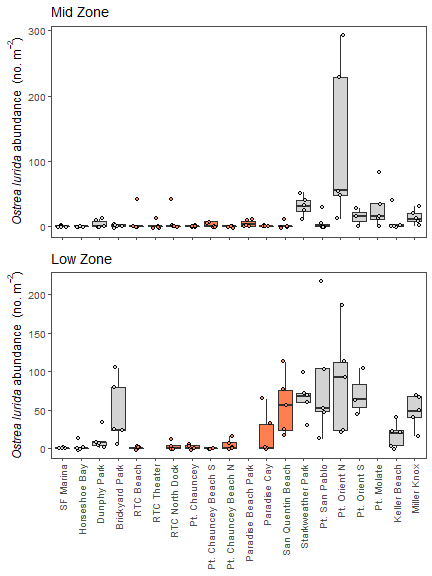
\includegraphics{sfb_quadrats_files/figure-latex/oysters-by-zone-site-fig-1} \hfill{}

\caption{ Native oyster (Ostrea lurida) abundance in the mid and low intertidal at survey sites. Colored fill indicates reference sites for RTC restoration planning.}\label{fig:oysters-by-zone-site-fig}
\end{figure}

\hypertarget{rockweed-by-site-type-and-zone}{%
\subsection{Rockweed by site type and zone}\label{rockweed-by-site-type-and-zone}}

\begin{figure}

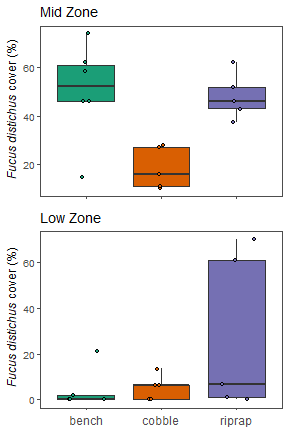
\includegraphics{sfb_quadrats_files/figure-latex/fucus-sitetype-zone-fig-1} \hfill{}

\caption{ Cover of rockweed (Fucus distichus) in the mid and low intertidal by site type.}\label{fig:fucus-sitetype-zone-fig}
\end{figure}

\hypertarget{oysters-by-site-type-and-zone}{%
\subsection{Oysters by site type and zone}\label{oysters-by-site-type-and-zone}}

\begin{figure}

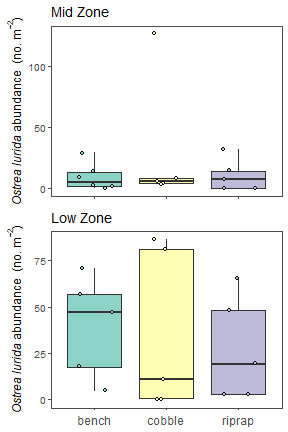
\includegraphics{sfb_quadrats_files/figure-latex/oysters-sitetype-zone-fig-1} \hfill{}

\caption{ Abundance of native oysters (Ostrea lurida) in the mid and low intertidal by site type.}\label{fig:oysters-sitetype-zone-fig}
\end{figure}

\hypertarget{oyster-scars-vs.-oysters-colored-by-site}{%
\subsection{Oyster scars vs.~oysters colored by site}\label{oyster-scars-vs.-oysters-colored-by-site}}

\begin{figure}

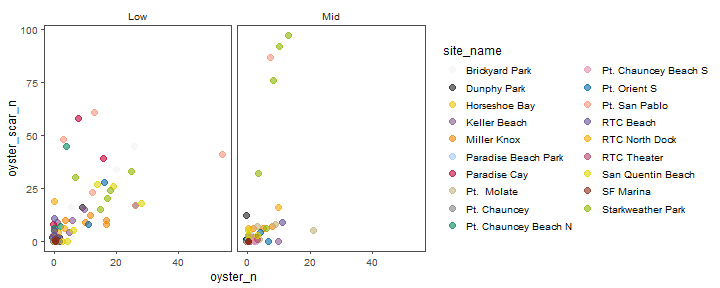
\includegraphics{sfb_quadrats_files/figure-latex/oyster-scar-plot-1} \hfill{}

\caption{ Abundance of native oysters (Ostrea lurida) in the mid and low intertidal by site type.}\label{fig:oyster-scar-plot}
\end{figure}

\hypertarget{size-structure-of-oysters-mussels-and-limpets-by-site}{%
\subsection{Size structure of oysters, mussels, and limpets by site}\label{size-structure-of-oysters-mussels-and-limpets-by-site}}

\begin{figure}

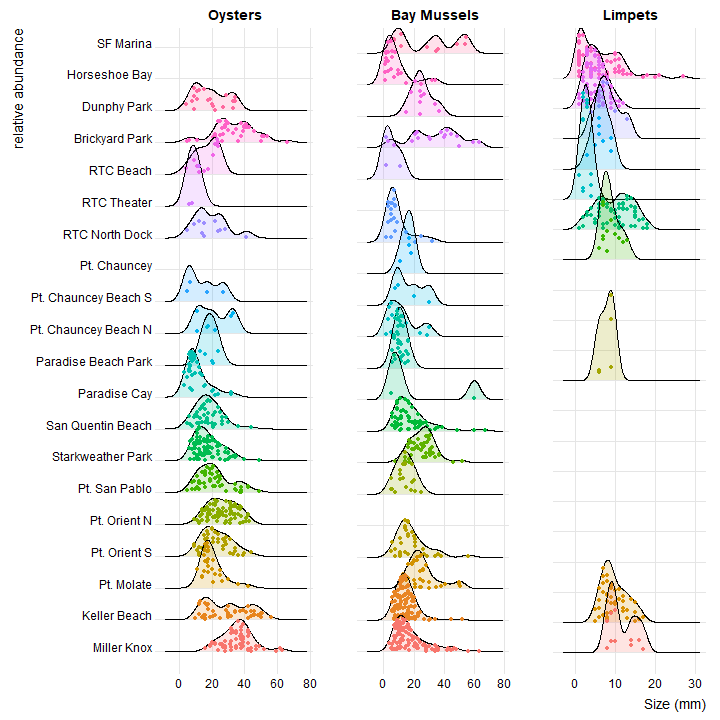
\includegraphics{sfb_quadrats_files/figure-latex/size-structure-plot-1} \hfill{}

\caption{ Size structure of oysters, bay mussels and limpets in mid and low intertidal at study sites.}\label{fig:size-structure-plot}
\end{figure}

\end{document}
